\documentclass[11pt, oneside]{article} 
\usepackage{geometry}
\geometry{letterpaper} 
\usepackage{graphicx}
	
\usepackage{amssymb}
\usepackage{amsmath}
\usepackage{parskip}
\usepackage{color}
\usepackage{hyperref}

\graphicspath{{/Users/telliott_admin/Tex/png/}}
% \begin{center} 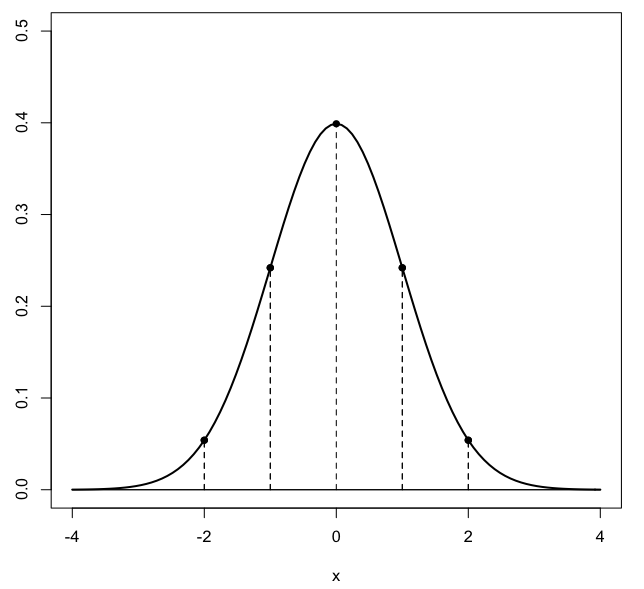
\includegraphics [scale=0.4] {gauss3.png} \end{center}

\title{Calculus:  introduction}
\date{}

\begin{document}
\maketitle
\Large

\label{sec:Calc_Intro}

You can understand the fundamental ideas in calculus by thinking about the instruments one uses in driving a car. Most drivers refer frequently to the speedometer (which measures velocity).  On the other hand, if they want to know about how far they've gone they refer to the odometer, which measures distance.

\begin{center} 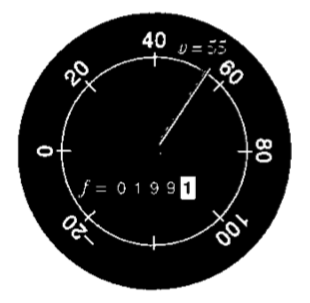
\includegraphics [scale=0.4] {Strang_speedometer.png} \end{center}

We'll use $s$ to refer to the distance traveled and $v$ for velocity.  If the velocity is constant and we start from $s = 0$ then:
\[ s = v \times t \]
Distance equals velocity times time. Travel at $60$ miles per hour for $2$ hours and you'll go $120$ miles.  

If we plot velocity as a \emph{function of time}, then for constant velocity the plot is a horizontal line.  Furthermore, the distance traveled is the \emph{area under the curve} (and above the $x$-axis).

For a car, imagine increasing the pressure on the gas pedal steadily so that after $1$ second you are going $10$ mph, after $2$ seconds $20$ mph, after $3$ seconds $30$ mph. If we continue at the same rate, we'll accelerate from $0$ to $60$ mph in $6$ seconds.



\end{document}